\documentclass[a4paper, 11pt]{article}
\usepackage[left=1.5cm, top=2.5cm, text={18cm, 25cm}]{geometry}
\usepackage[slovak]{babel}
\usepackage[T1]{fontenc}
\usepackage[utf8]{inputenc}
\usepackage{times}
\usepackage[unicode]{hyperref}
%\usepackage{stackrel}
\usepackage{array}
\usepackage{graphicx}
\usepackage{graphics}



\title{
\includegraphics[scale=0.1,keepaspectratio]{./src/latex/pics/logo_cz.eps}\\Užívateľská dokumentácia}
\author{Tím G.I.I.T.}
\date{\today}

\begin{document}
	\maketitle
	\tableofcontents
	\newpage
	
    \section{Úvod}
    V tomto návode nájdete informácie ako ovládať kalkulačku a tiež aj informácie o každej jej funkcií.\\
    Ďakujeme, že používate našu kalkulačku. \\
    Táto kalkulačka bolo vytvorená ako vysokoškolský projekt. 
    \section{Predispozície}
    \begin{itemize}
        \item python3.7+
        \item Operačný systém Ubuntu 20.04+
    \end{itemize}
    \section{Inštalácia a odinštalácia}
    \subsection{Nainštalovanie}
    \begin{itemize}
        \item pomocou .deb súboru
        \begin{itemize}
            \item pre nainštalovanie kalkulačky kliknite na .deb súbor pravým a vyberte Ubuntu package manager
        \end{itemize}
        \item pomocou terminálu
        \begin{itemize}
            \item otvorte terminál a zadajte \texttt{ sudo dpkg -i giit-calc-1.0\_amd64.deb }
        \end{itemize}
        \item súbor bude nainštalovaný v \texttt{ usr/opt/giit-calc }
    \end{itemize}
    \subsection{Odinštalovanie}
    \begin{itemize}
        \item pomocou .deb súbor pravým a vyberte
        \begin{itemize}
            \item je potreba nájsť adresáre \texttt{ /usr/bin/giit-calc } a \texttt{ /usr/opt/giit-calc }a odstrániť ich
        \end{itemize}
        \item pomocou terminálu
        \begin{itemize}
            \item otvorte terminál a zadajte \texttt{ sudo dpkg --purge giit-calc }
        \end{itemize}
    \end{itemize}
    \newpage
    \section{Ako pracovať s programom}
    \subsection{Rozloženie aplikácie}
    \begin{figure}[!h]
        \centering
        \scalebox{0.5}{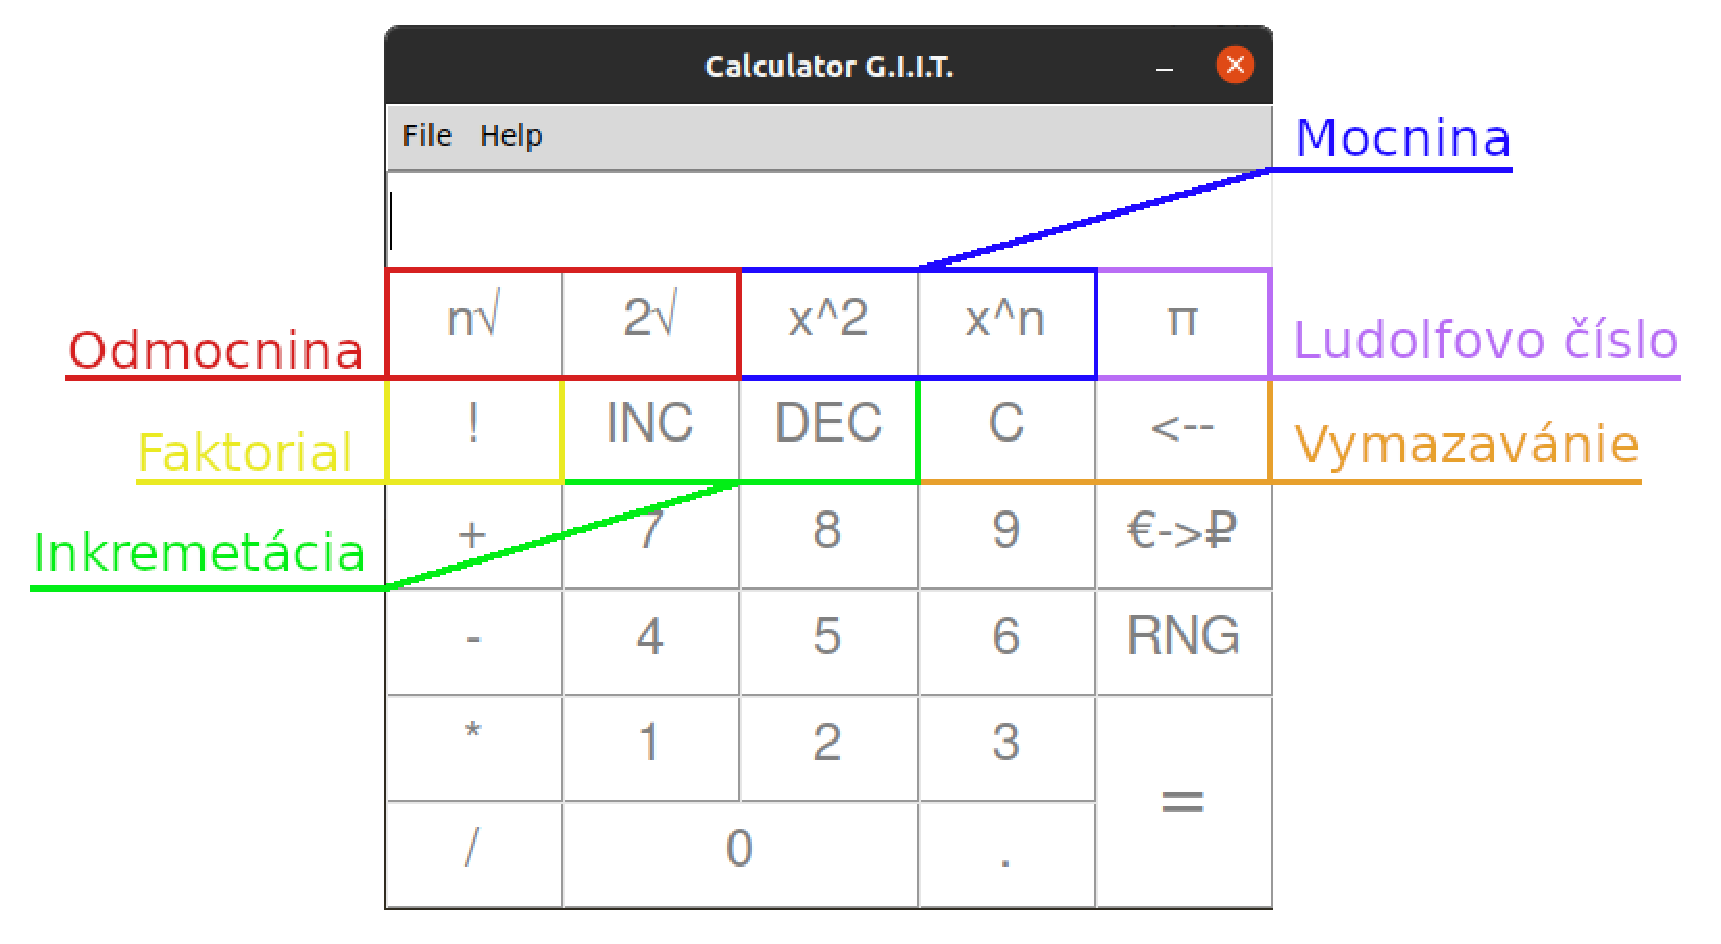
\includegraphics{./src/latex/pics/top.eps}}
        \caption{Vrchná časť kalkulačky}
        \label{fig:obrazok1}
    \end{figure}
    
    \begin{figure}[!h]
        \centering
        \scalebox{0.5}{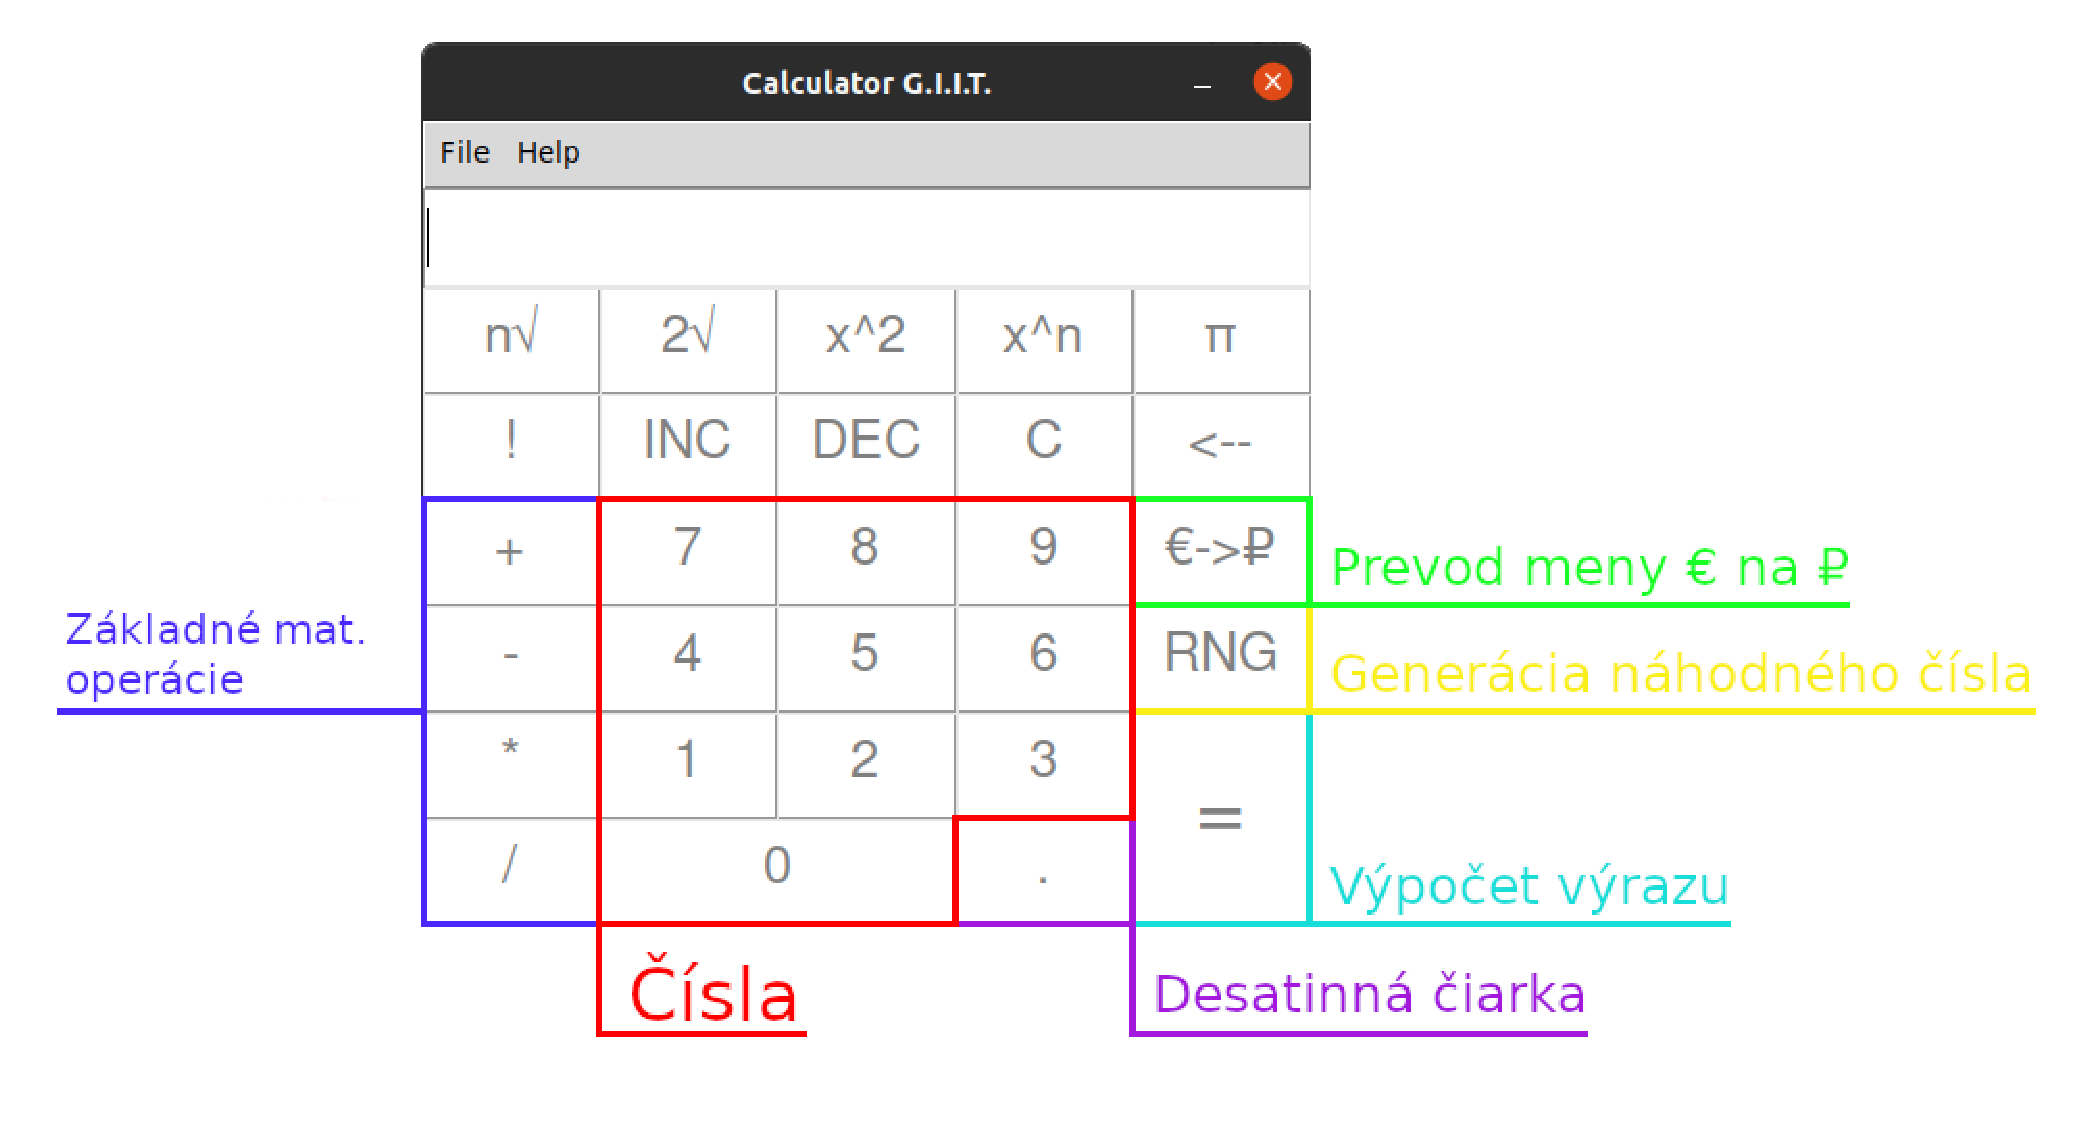
\includegraphics{./src/latex/pics/bottom.eps}}
        \caption{Spodná časť kalkulačky}
        \label{fig:obrazok2}
    \end{figure}
    
    \begin{itemize}
        \item v menu \emph{File} je možné ukončiť aplikáciu
        \item v menu \emph{Help} je možné nájsť odkaz na manuál a informácie o aplikácií
    \end{itemize}
    \newpage
    \subsection{Operácie}
    \begin{center}
    \begin{tabular}{ |c|c|c|c| } 
         \hline
         \textbf{Operácia} & \textbf{Príklad zápisu} & \textbf{Tlačidlo} & \textbf{Klávesa} \\ \hline
         Sčítanie &  $5+4$ & + & + \\ \hline
         Odčítanie & $5-4$ & - & - \\ \hline
         Násobenie & $5*4$ & * & *\\ \hline
         Delenie & $5/4$ & / & / \\ \hline
         Generácia náhodného čísla & NONE & NONE & RNG\\ \hline
         Mocnina & $5{\mathchar"5E}4$ & ${\mathchar"5E}$ & ${\mathchar"5E}$\\ \hline
         Odmocnina & $5 \sqrt 4$ & NONE & NONE\\ \hline
         Faktorial & $ 5! $ & ! & !\\ \hline
         Inkrement & $inc5$ & INC & NONE \\ \hline
         Dekrement & $dec5$ & DEC & NONE\\ \hline
         Ludolfovo číslo & e & e & e\\ \hline
         Eulerovo číslo & $\pi$ & $\pi$ & NONE\\ \hline
         Výpočet výrazu & NONE & = & Enter\\ \hline
         Zmazanie posledného znaku & NONE & <-- & BackSpace\\ \hline
         Zmazanie celého výrazu & NONE & C & NONE \\ \hline
    \end{tabular}
    \end{center}
    \begin{itemize}
        \item Základné matematické operácie
        \begin{itemize}
            \item sčítanie (+)
            \item odčítanie (-)
            \item násobenie (*)
            \item delenie (/)
        \end{itemize}
        \item Generácia náhodného čísla
        \begin{itemize}
            \item vygenerovanie náhodného čísla pre ďalšie výpočty
        \end{itemize}
        \item Odmocniny a mocniny
        \begin{itemize}
            \item je možné zadať priamo druhú mocninu/odmocninu alebo vybrať vlastnú
        \end{itemize}
        \item Inkrementácia
        \begin{itemize}
            \item inkrement (INC)
            \begin{itemize}
                \item zvýši hodnotu čísla o 1
            \end{itemize}
            \item dekrement (DEC)
            \begin{itemize}
                \item zníži hodnotu čísla o 1
            \end{itemize}
        \end{itemize}
    \end{itemize}
    \newpage
    \subsection{Všeobecné informácie}
    \begin{itemize}
        \item kalkulačku je možné ovládať pomocou klávesnice aj myšky
        \item s výsledkom je možné aj po výpočte ďalej pracovať
        \item všetky výsledky dlhšie ako 16 znakov sú prevedené do exponecialného zápisu
        \item kalkulačka podporuje Ludolfovo aj Eulerovo číslo
        \item nie je možné vymazať výraz označením čísla ani presunúť kurzor pomocou myšky
    \end{itemize}
    \subsection{Typy chýb}
    \begin{itemize}
        \item Arithmetic error
        \begin{itemize}
            \item spôsobené matematickou chybou
            \item delenie nulou, párna odmocnina záporného čísla, faktorial desatinného a záporného čísla
        \end{itemize}
        \item Syntax error
        \begin{itemize}
            \item zlý zápis matematických výrazov
            \item napr. '$5*/8$', '$5+$', '$!5$' atď.
        \end{itemize}
    \end{itemize}
\end{document}
